\documentclass{article}
\usepackage{amsmath}
\usepackage{amssymb}
\usepackage{enumitem}
\usepackage{algorithm}
\usepackage{listings}
\usepackage{color,xcolor}
\usepackage[T1]{fontenc}
\usepackage{etoolbox}
\usepackage{multicol}
\usepackage{geometry}
\usepackage[colorlinks=true,linkcolor=blue,urlcolor=red,bookmarksopen=true]{hyperref}
\usepackage{tikz, pgfplots, tkz-euclide,calc}
    \usetikzlibrary{patterns,snakes,shapes.arrows,3d,patterns.meta,angles,quotes}
    \geometry{
        total = {160mm, 237mm},
        left = 25mm,
        right = 35mm,
        top = 30mm,
        bottom = 30mm,
      }

\usepackage{tcolorbox}
     \tcbuselibrary{listings,skins}

\newcommand{\enter}{\raisebox{-1.8pt}{
\begin{tikzpicture}[scale=0.3]
    \draw[thin,fill=lightgray] (0,0) rectangle (2,1);
    \draw (0.3,0.3) -- (0.7,0.3)--(0.7,0.6);     
\end{tikzpicture}}}

\definecolor{HIMAmuda}{HTML}{01D1FD}
\definecolor{HIMAtua}{HTML}{02016A}
\definecolor{HIMAabu}{HTML}{CBCBCC}
\definecolor{pgray}{rgb}{0.5,0.5,0.5}
\definecolor{pblue}{rgb}{0.13,0.13,1}
\definecolor{pgreen}{rgb}{0,0.5,0}
\definecolor{pred}{rgb}{0.9,0,0}
\definecolor{pgrey}{rgb}{0.46,0.45,0.48}
\definecolor{pcyan}{HTML}{D4EFFC}
\definecolor{lblue}{HTML}{00AEEF}
\definecolor{input}{HTML}{AAE1FA}
\definecolor{bg}{rgb}{0.95, 0.95, 0.92}
\definecolor{vscode}{HTML}{282A36}
\definecolor{PastelGreen}{HTML}{77DD77}

\newcommand{\inputscan}[1]{\raisebox{0pt}[1pt]{\colorbox{darkgray}{#1}}}

\usepackage{listings}

\lstdefinestyle{Liang}{
language=Java,
showspaces=false,
showtabs=false,
breaklines=true,
showstringspaces=false,
breakatwhitespace=true,
commentstyle=\color{pgray},
keywordstyle=\color{pblue},
stringstyle=\color{pgreen},
basicstyle=\small\ttfamily,
frame=single,
backgroundcolor=\color{pcyan},
escapeinside={(*}{*)},}

\lstdefinestyle{output}{
    language=Java,
    backgroundcolor=\color{vscode},
    basicstyle=\small\ttfamily\color{white},
    frame=none,
    escapeinside={(*}{*)},
    showspaces=false,
    showtabs=false,
    breaklines=true,
    showstringspaces=false,
    breakatwhitespace=true,
    keywordstyle=\color{white},
    }

\lstdefinestyle{standard}{
    language=Java,
    showspaces=false,
    showtabs=false,
    breaklines=true,
    showstringspaces=false,
    breakatwhitespace=true,
    commentstyle=\color{pgray},
    keywordstyle=\color{pblue},
    stringstyle=\color{pgreen},
    basicstyle=\small\ttfamily,
    frame=single,
    backgroundcolor=\color{bg},
    escapeinside={(*}{*)},}
\lstset{style=Liang}

\newtcblisting{RunCode}[1][enhanced,drop shadow]{
    arc=0pt, outer arc=0pt,
    boxsep=1pt,
    boxrule=2pt,
    auto outer arc,
    colback=vscode,
    colframe=bg,
    listing only, 
    listing style=output,
    title=\color{black}Ex. Output,
    #1
    }

\newtcolorbox{hint}[1][]{
    colback=PastelGreen!5!white, 
    colframe=PastelGreen!75!black,
    fonttitle=\bfseries, 
    colbacktitle=PastelGreen!85!black,
    enhanced, 
    attach boxed title to top left={yshift=-2mm}, 
    title=Hint,
    #1
}

\newtcolorbox{req}[1][]{
    colback=lblue!5!white, 
    colframe=lblue!75!black,
    fonttitle=\bfseries, 
    colbacktitle=lblue!85!black,
    enhanced, 
    attach boxed title to top left={yshift=-2mm}, 
    title=Input,
    #1
}

\newtcolorbox{out}[1][]{
    colback=HIMAtua!5!white, 
    colframe=HIMAtua!75!black,
    fonttitle=\bfseries, 
    colbacktitle=HIMAtua!85!black,
    enhanced, 
    attach boxed title to top left={yshift=-2mm}, 
    title=Output,
    before upper=\renewcommand\thempfootnote{\Roman{mpfootnote}},
    #1
}

\renewcommand{\thesubsection}{\arabic{subsection}}
\newcommand{\R}{\mathbb{R}}
\newcommand{\Z}{\mathbb{Z}}

\title{\textbf{Week 3 Assigment}}
\date{23 September 2024}
\author{Teosofi H.A \& Hafidz M.}

\begin{document}
    \maketitle
    \pagenumbering{gobble}

    \section*{Tugas Mandiri}
    \begin{enumerate}[label=\textbf{\arabic*.}]
        \item \textbf{(Geometri Analitik)}\\
        Buatlah program untuk menghitung jarak dari titik $(x_0,y_0)$ ke garis lurus $ax+by+c=0$.
        \begin{req}
            \begin{itemize}
                \item $-50\leq x_0,y_0\leq 50,\quad x_0,y_0\in\Z$
                \item $0 \leq a,b,c\leq 10,\quad a,b,c\in\Z$
            \end{itemize}
        \end{req}
        \begin{out}
            \begin{itemize}
                \item $d:=$ Jarak titik ke garis\footnote{Cukup tampilkan 2 angka di belakang koma}\\
                $d\geq 0,\quad d\in\R$
            \end{itemize}      
        \end{out}
        \begin{hint}
            Gunakan \texttt{Math.abs()} untuk menghitung nilai mutlak.
        \end{hint}
        \begin{RunCode}
Masukkan titik (x0,y0): (*\inputscan{1 2} \enter*) 
Masukkan koefisien garis (a,b,c): (*\inputscan{1 1 0} \enter*)
Jarak titik (1,2) ke garis adalah 2.12
        \end{RunCode}

        \newpage
        \item \textbf{(Fisika Mekanika)}\\
        Sebuah bola dilempar dari Lantai-4 Lab Provikom dengan ketinggian 12 meter dari tanah. Kecepatan awal bola adalah $v_0$ (dalam $m/s$) dan sudut lemparan adalah $\theta$ (dalam derajat) terhadap vertikal ke atas. Asumsikan percepatan gravitasi adalah $9.8$ $m/s^2$.
        \begin{center}
            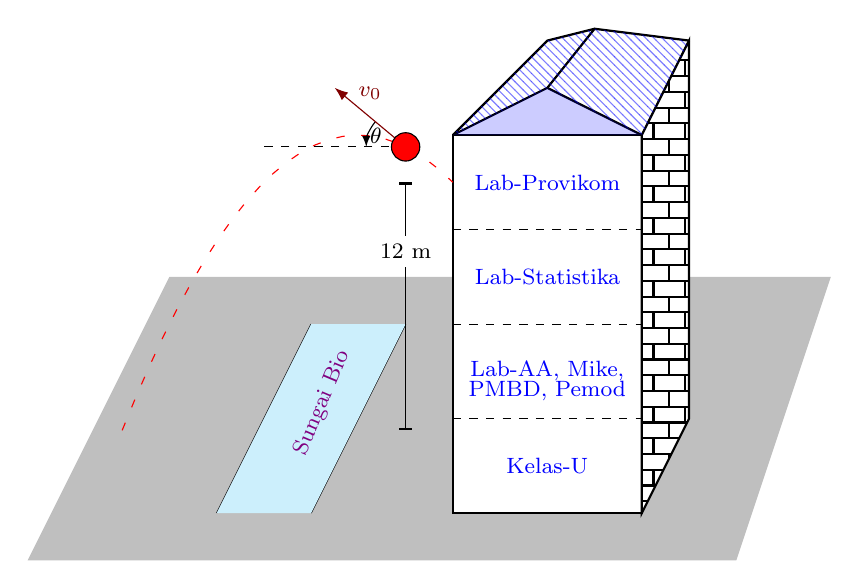
\begin{tikzpicture}[scale=1.2]
                \fill[lightgray] (-4.5,-0.5) -- (-3,2.5) -- (4,2.5) -- (3,-0.5) -- cycle;

                \draw[thick,fill=white] (0,4) -- (1,4.5) -- (2,4) -- (2.5,5);
                \draw[thick,fill=white] (0,4) -- (1,5) -- (1.5,5.125);
                \draw[thick,fill=white] (1,4.5) -- (1.5,5.125) -- (2.5,5);
                \draw[thick,fill=white] (0,0) -- (0,4) -- (2,4) -- (2,0) -- cycle;
                \draw[thick,fill=white] (2,0) -- (2.5,1) -- (2.5,5) -- (2,4) -- cycle;

                \fill[pattern={bricks[rotate=45]}] (2,.0) -- (2.5,1) -- (2.5,5) -- (2,4) -- cycle;
                \fill[pattern={north west lines},pattern color=blue,opacity=0.5] (0,4) -- (1,4.5) -- (2,4) -- (2.5,5) -- (1.5,5.125) -- (1,5) -- cycle;
                \fill[blue,opacity=0.2] (0,4) -- (1,4.5) -- (2,4) -- cycle;

                \draw (1,3.5) node[] {\footnotesize\color{blue} Lab-Provikom};
                \draw[dashed] (0,3) -- (2,3);
                \draw (1,2.5) node[] {\footnotesize\color{blue} Lab-Statistika};
                \draw[dashed] (0,2) -- (2,2);
                \draw (1,1.5) node[] {\footnotesize\color{blue} Lab-AA, Mike,};
                \draw (1,1.5) node[below] {\footnotesize\color{blue} PMBD, Pemod};
                \draw[dashed] (0,1) -- (2,1);
                \draw (1,0.5) node[] {\footnotesize\color{blue} Kelas-U};

                \draw (-1.5,0) -- (-0.5,2); 
                \draw (-2.5,0) -- (-1.5,2);
                \fill[cyan!20] (-1.5,0) -- node[midway,rotate=67,yshift=0.5cm,violet]{\footnotesize Sungai Bio} (-0.5,2) -- (-1.5,2) -- (-2.5,0) -- cycle;

                \draw[loosely dashed,red,domain=-3.5:0] plot (\x,{-1/2*(\x+1)^2+4});
                \draw[white] (-1.25,4.5) coordinate (A) -- (-0.5,3.875) coordinate (B) -- (-2,3.875) coordinate (C) pic [black,"\footnotesize$\theta$", draw, -latex,angle eccentricity=0.8] {angle};
                \draw[-||] (-0.5,2.5) -- (-0.5,0.875);
                \draw[-||] (-0.5,2.5) node[above]{\colorbox{white}{\footnotesize$12$ m}} -- (-0.5,3.5);
                \draw[red!50!black,-Latex] (-0.5,3.875) -- (-1.25,4.5) node[midway,above,yshift=1mm] {\footnotesize $v_0$};
                \draw[dashed] (-0.5,3.875) -- (-2,3.875);
                \draw[fill=red] (-0.5,3.875) circle (0.15);
            \end{tikzpicture}
        \end{center}
        Buatlah program untuk menghitung waktu bola sampai ke tanah dan jarak horizontal bola dari titik lemparan.
        \begin{req}
            \begin{itemize}
                \item $0\leq v_0\leq 100,\quad v_0\in\R$
                \item $0\leq \theta\leq 90^\circ,\quad \theta\in\R$
            \end{itemize}
        \end{req}
        \begin{out}
            \begin{itemize}
                \item $t:=$ Waktu bola sampai ke tanah dalam satuan detik\footnote{Cukup tampilkan 4 angka di belakang koma}\\
                $t\geq 0,\quad t\in\R$
                \item $s_x:=$ Jarak horizontal bola dari titik lemparan dalam satuan meter\footnote{Cukup tampilkan 3 angka di belakang koma}\\
                $s_x\geq 0,\quad s_x\in\R$
            \end{itemize}
        \end{out}
        \begin{hint}
            \begin{itemize}
                \item Gunakan \texttt{Math.sin()} dan \texttt{Math.cos()} untuk menghitung nilai sinus dan cosinus.
                \item Untuk mengkonversi sudut dari derajat ke radian, gunakan \texttt{Math.toRadians()}.
                \item Untuk mencari akar kuadrat, gunakan \texttt{Math.sqrt()}.
            \end{itemize}
        \end{hint}
        \begin{RunCode}
Masukkan kecepatan awal : (*\inputscan{10} \enter*)
Masukkan sudut lemparan : (*\inputscan{30} \enter*)
Waktu bola sampai ke tanah adalah 2.1562 detik
Jarak horizontal bola dari titik lemparan adalah 18.673 meter
        \end{RunCode}
    \end{enumerate}
\end{document}